\section{Grafer og grafalgoritmer}
Det er tre måter å traversere et binært tre på; preorder, inorder og postorder.
\begin{itemize}
    \item \textbf{Preorder}: Her printer man ut nodens verdi før dens barn, venstre og deretter høyre. 
    \begin{itemize}
        \item Eksempel fra figuren under: 10, 6, 3, 2, 1, 4, 5, 8, 7, 9, 13, 11, 12, 18, 15, 14, 16, 17
    \end{itemize}
    \item \textbf{Inorder}: Her printer man venstre barn, noden, og deretter høyre barn (om ikke det er noe venstre barn, print noden før høyre barn)
    \begin{itemize}
        \item Eksempel fra figuren under: 1, 2, 3, 4, 5, 6, 7, 8, 9, 10, 11, 12, 13, 14, 15, 16, 17, 18
    \end{itemize}
    \item \textbf{Postorder}: Her printer man nodens verdi etter man har printet venstre og høyre barn
    \begin{itemize}
        \item Eksempel fra figuren under: 1, 2, 5, 4, 3, 7, 9, 8, 6, 12, 11, 14, 17, 16, 15, 18, 13, 10
    \end{itemize}
\end{itemize}

\begin{figure}[H]
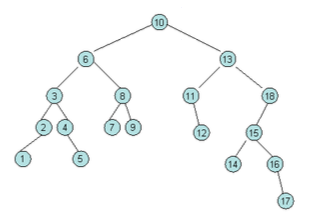
\includegraphics[scale=0.7]{images/tregraf}
\centering %centering the image
\caption{Tre}
\label{fig:tregraf}
\end{figure}

\subsection{Representasjon}
\subsubsection{Nabolister}
\subsubsection{Nabomatriser}
\subsection{Traversering}
\subsubsection{Bredde-først-søk (BFS)}
BFS implementeres med en kø. BFS utforsker grafen i bredden. Man starter på foreldrenoden og legger inn alle dens barn i køen. Når alle naboer til node $x$ er oppdaget, fjernes den fra køen og man tar den neste noden i køen og legger alle dens barn inn i køen. Når køen er tom, sjekker man ikke videre om det er ubesøkte noder.

\begin{lstlisting}
    function BFS(G,v) // v er startnode
	    lag en kø Q
    	legg v inn i Q
    	while Q.notEmpty() do
    		v = Q.dequeue()
    		for each edge e adjacent to v do
    			if e not marked then
    				mark w
    				Q.enqueue(e)
    			end if
    		end for
    	end while
    end function

\end{lstlisting}


\noindent \textbf{Traversering}

\subsubsection{Dybde-først-søk (DFS)}
DFS implementeres med en stack. DFS utforsker grafen i dybden. Den fyller stacken med noder den støter på. Kan man ikke gå videre vil den “backtrace” til forrige node og se etter en mulig vei videre. Hvis stacken er tom, sjekker man om alle noder er besøkt. Hvis ikke, starter man på nytt fra ubesøkte noder.

\begin{lstlisting}
    function DFS(G,v)	//v er startnode
	    initialiser en tom stack, S
    	for each vertex u in G do
    		set visited[u] $\rightarrow$ false
    	end for
    	S.push(v)
    	while S.notEmpty() do
    		u = S.pop()
    		for all w adjacent to u do
    			if not visited[w] then
    				visited[w] $\rightarrow$ true
    				S.push(w)
    			end if
    		end for
    	end while
    end function
\end{lstlisting}

\noindent \textbf{Traversering}

\subsection{Korteste vei}
\subsubsection{En til alle}
\textbf{Dijkstras algoritme}\\
Dijkstra er en korteste vei, en-til-alle-algoritme. Tillater ikke negative kanter. Den velger noder en etter en fra hvor nærme de er startnoden. Dijkstra er en grådig algoritme.

\begin{lstlisting}
    function DIJKSTRA(G,w,s)
	    INITIALIZE-SINGLE-SOURCE(G,s)
    	S = Ø
    	Q = G.V
    	while Q $\neq$ Ø do
    		u = EXTRACT-MIN(Q)
    		S = S $\cup$ {u}
    		for each vertex v $\in$ G.Adj[u] do
    			RELAX(u,v,w)
    		end for
    	end while
    end function
\end{lstlisting}

\textbf{Bellman-ford}\\
\textbf{DAG shortest path}\\
DAG-Shortest-Path er en korteste vei, en-til-alle algoritme. Tillater ikke negative kanter, og kan selvfølgelig ikke ha sykler, da det er en DAG. Gjør topologisk sortering av DAGen og besøker hver node en gang for å kjøre RELAX på nodene foran.

\begin{lstlisting}
    function DAG-SHORTEST-PATH(G,w,s)
    	TOPOLOGICAL-SORT(G)
    	INITIALIZE-SINGLE-SOURCE(G,s)
    	for each vertex u, taken in topologically sorted order do
    		for each vertex v ∈ G.Adj[u] do
    			RELAX(u,v,w)
    		end for
    	end for
    end function

\end{lstlisting}

\subsubsection{Alle til alle}
\textbf{Floyd-Warshall}\\
Floyd-Warshall er en korteste vei, alle-til-alle-algoritme. Den bruker DP. Lager en nabomatrise for alle noder og hvor det går kantvekter. Konstanden mellom disse blir verdien av kanten. Er det ikke en direkte vei mellom to noder settes verdien til $\infty$. Deretter velger den en node a og sjekker om veien fra u til v er kortere via a. Deretter finner den en ny node, og sjekker om det er kortere veier om man benytter seg av denne. Slik fortsetter den til den har besøkt alle noder.

\subsection{Maksimal flyt}
\subsubsection{Flytnettverk}
\subsubsection{Residualnettverk}
\subsubsection{Flytforøkende sti}
\subsubsection{Minimalt kutt}
Minimum-snitt (min-cut) på et flytnettverk: det snittet som har lavest kapasitet av alle snitt. Det vil si min-cut angir en flaskehals i flytnettverket. Det vil si at det ikke kan sendes mer flyt gjennom nettverket enn det vi kan sende gjennom flaskehalsen. Man kan da ikke finne noen flytforøkende sti over flaskehalsen. Det vil da være maksimal-flyt, max-flow.\\

\noindent \textbf{Ford-Fulkersons metode}\\
Ford-Fulkerson-metoden finner maksimal flyt i et flytnettverk. Hver iterasjon forsøker å finne en flytforøkende sti, og setter på all den flyten som er mulig. Deretter leter den etter en ny flytforøkende sti, og gjentar prosessen. Når det ikke er flere flytforøkende stier har man oppnådd maksimal flyt. Den benytter seg av DFS for å finne flytforøkende sti.
\\

\noindent \textbf{Edmonds-Karp}\\
Endret en bokstav på Ford-Fulkerson-metoden. De benytter seg av BFS. Edmonds-Karp bruker Ford-Fulkerson og BFS til å finne flytforøkende stier.\\